\subsection{User Interfaces}
DREAM contains 2 main interfaces: mobile application and website interface.
In both interfaces, all 3 actors can perform the same operations, from a mobile interface and from a website.
However, it should be noted that certain features are more comfortable to use only from a certain interface.
The following mockups will give a more detailed description in terms of interfaces.

\begin{figure}[H]
  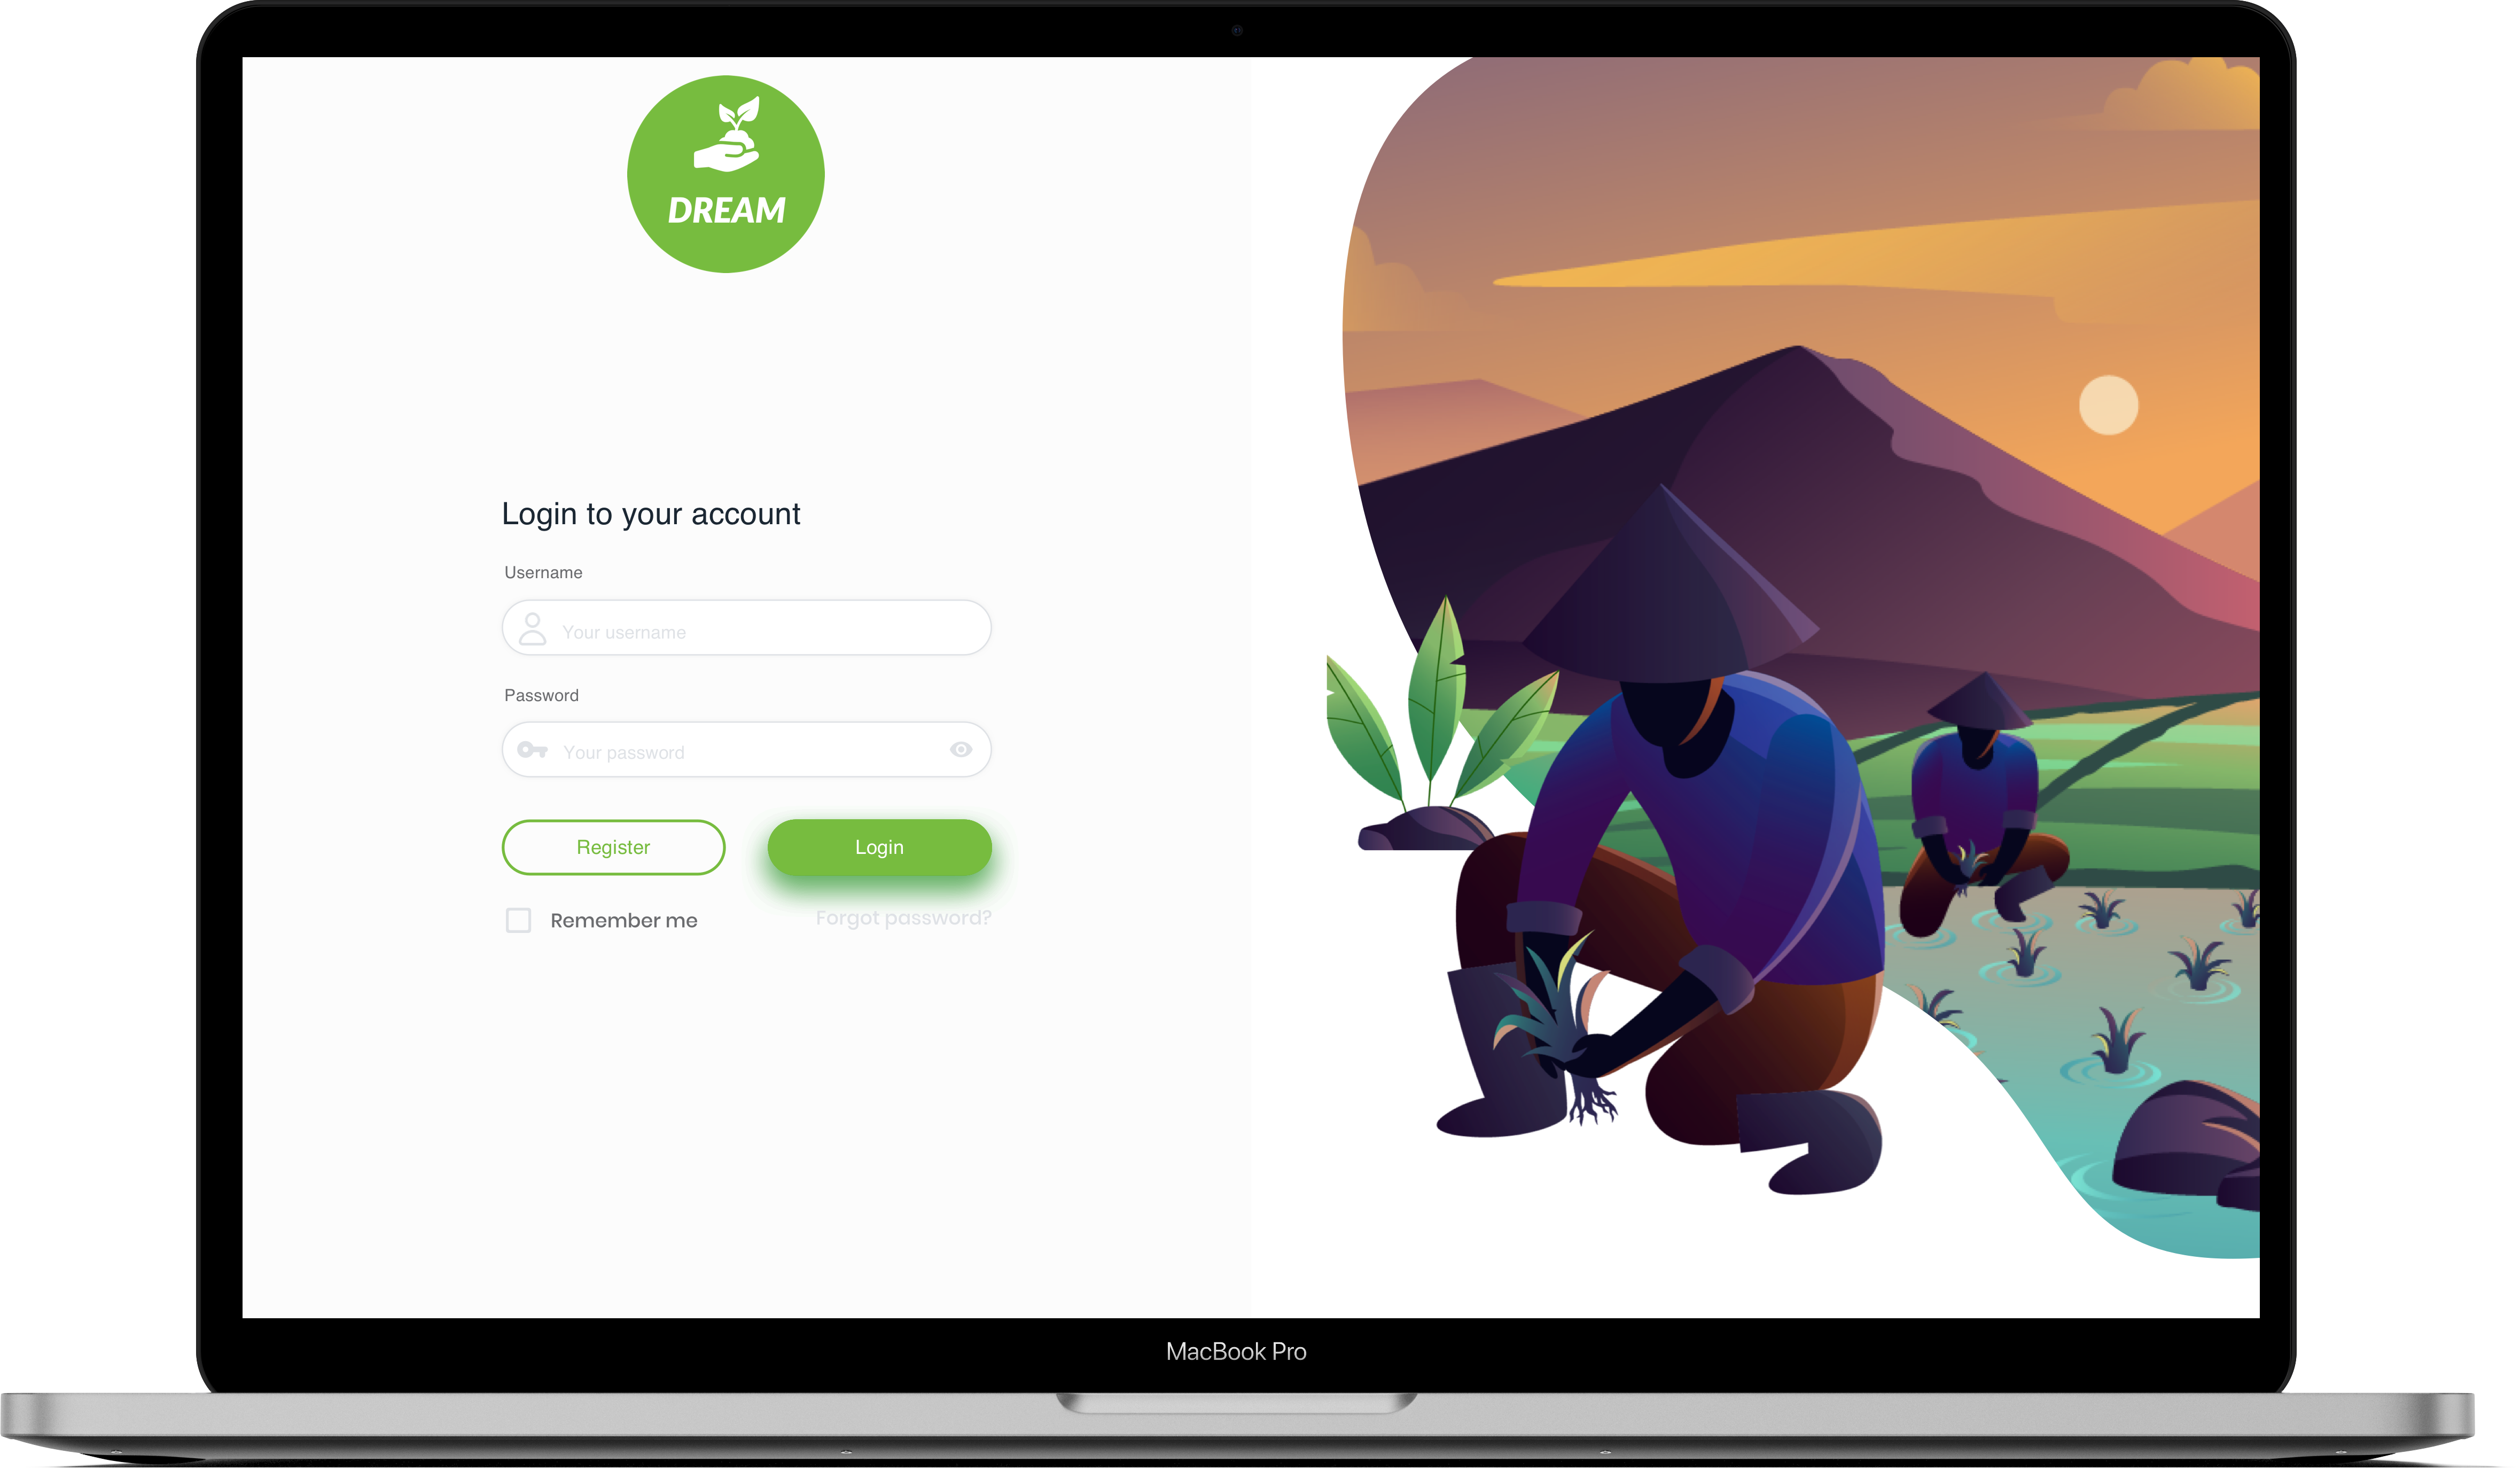
\includegraphics[width=140mm,scale=0.9]{./Images//Mocks/WebApp/Login.png}
  \caption{Login}
\end{figure}

\begin{itemize}
    \item \textbf{Website Login}\\ 
    \textcolor{red}{The 3 actors of DREAM can access to the application through this login page. If they do not yet have an account, they can simply access the registration page via an appropriate button}
\end{itemize}


\begin{figure}[H]
  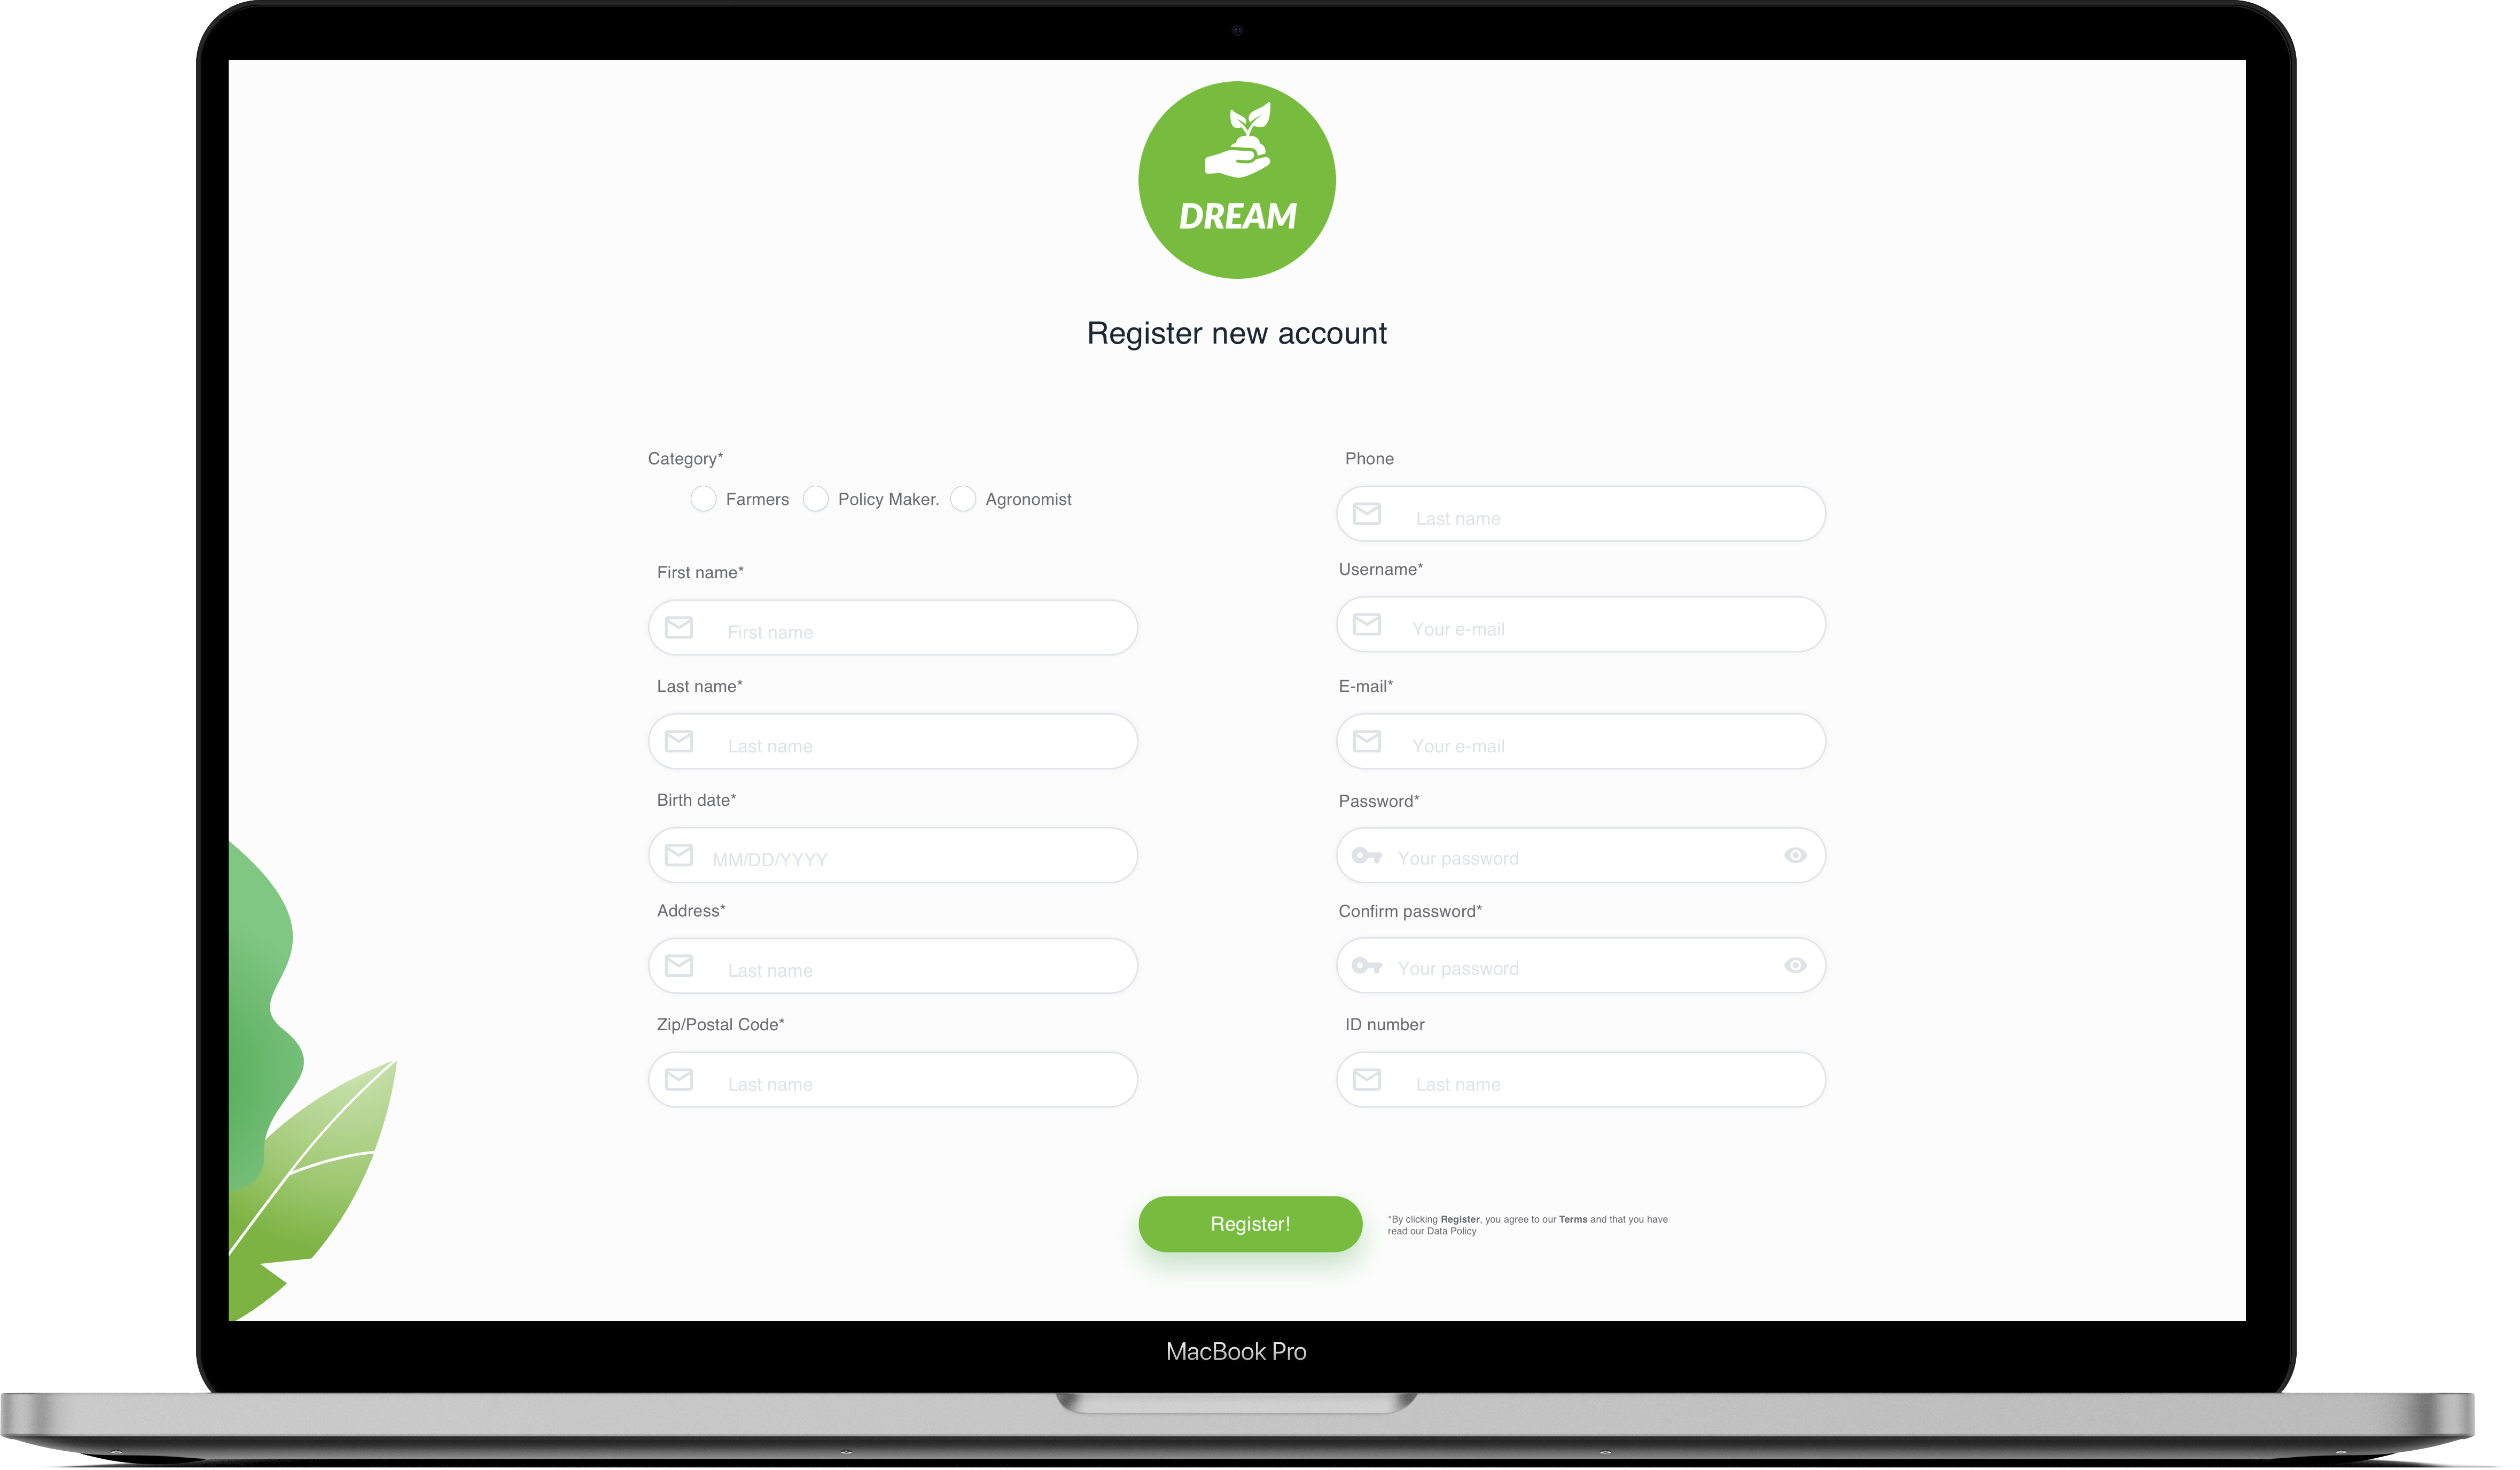
\includegraphics[width=140mm,scale=0.9]{./Images//Mocks/WebApp/Registration.png}
  \caption{Registration}
\end{figure}

\begin{itemize}
    \item \textbf{Website Registration}\\ 
    \textcolor{red}{The 3 actors can register to DREAM through this registration page, where there are some required fields, and registration is completed by accepting term and conditions}
\end{itemize}


\begin{figure}[H]
  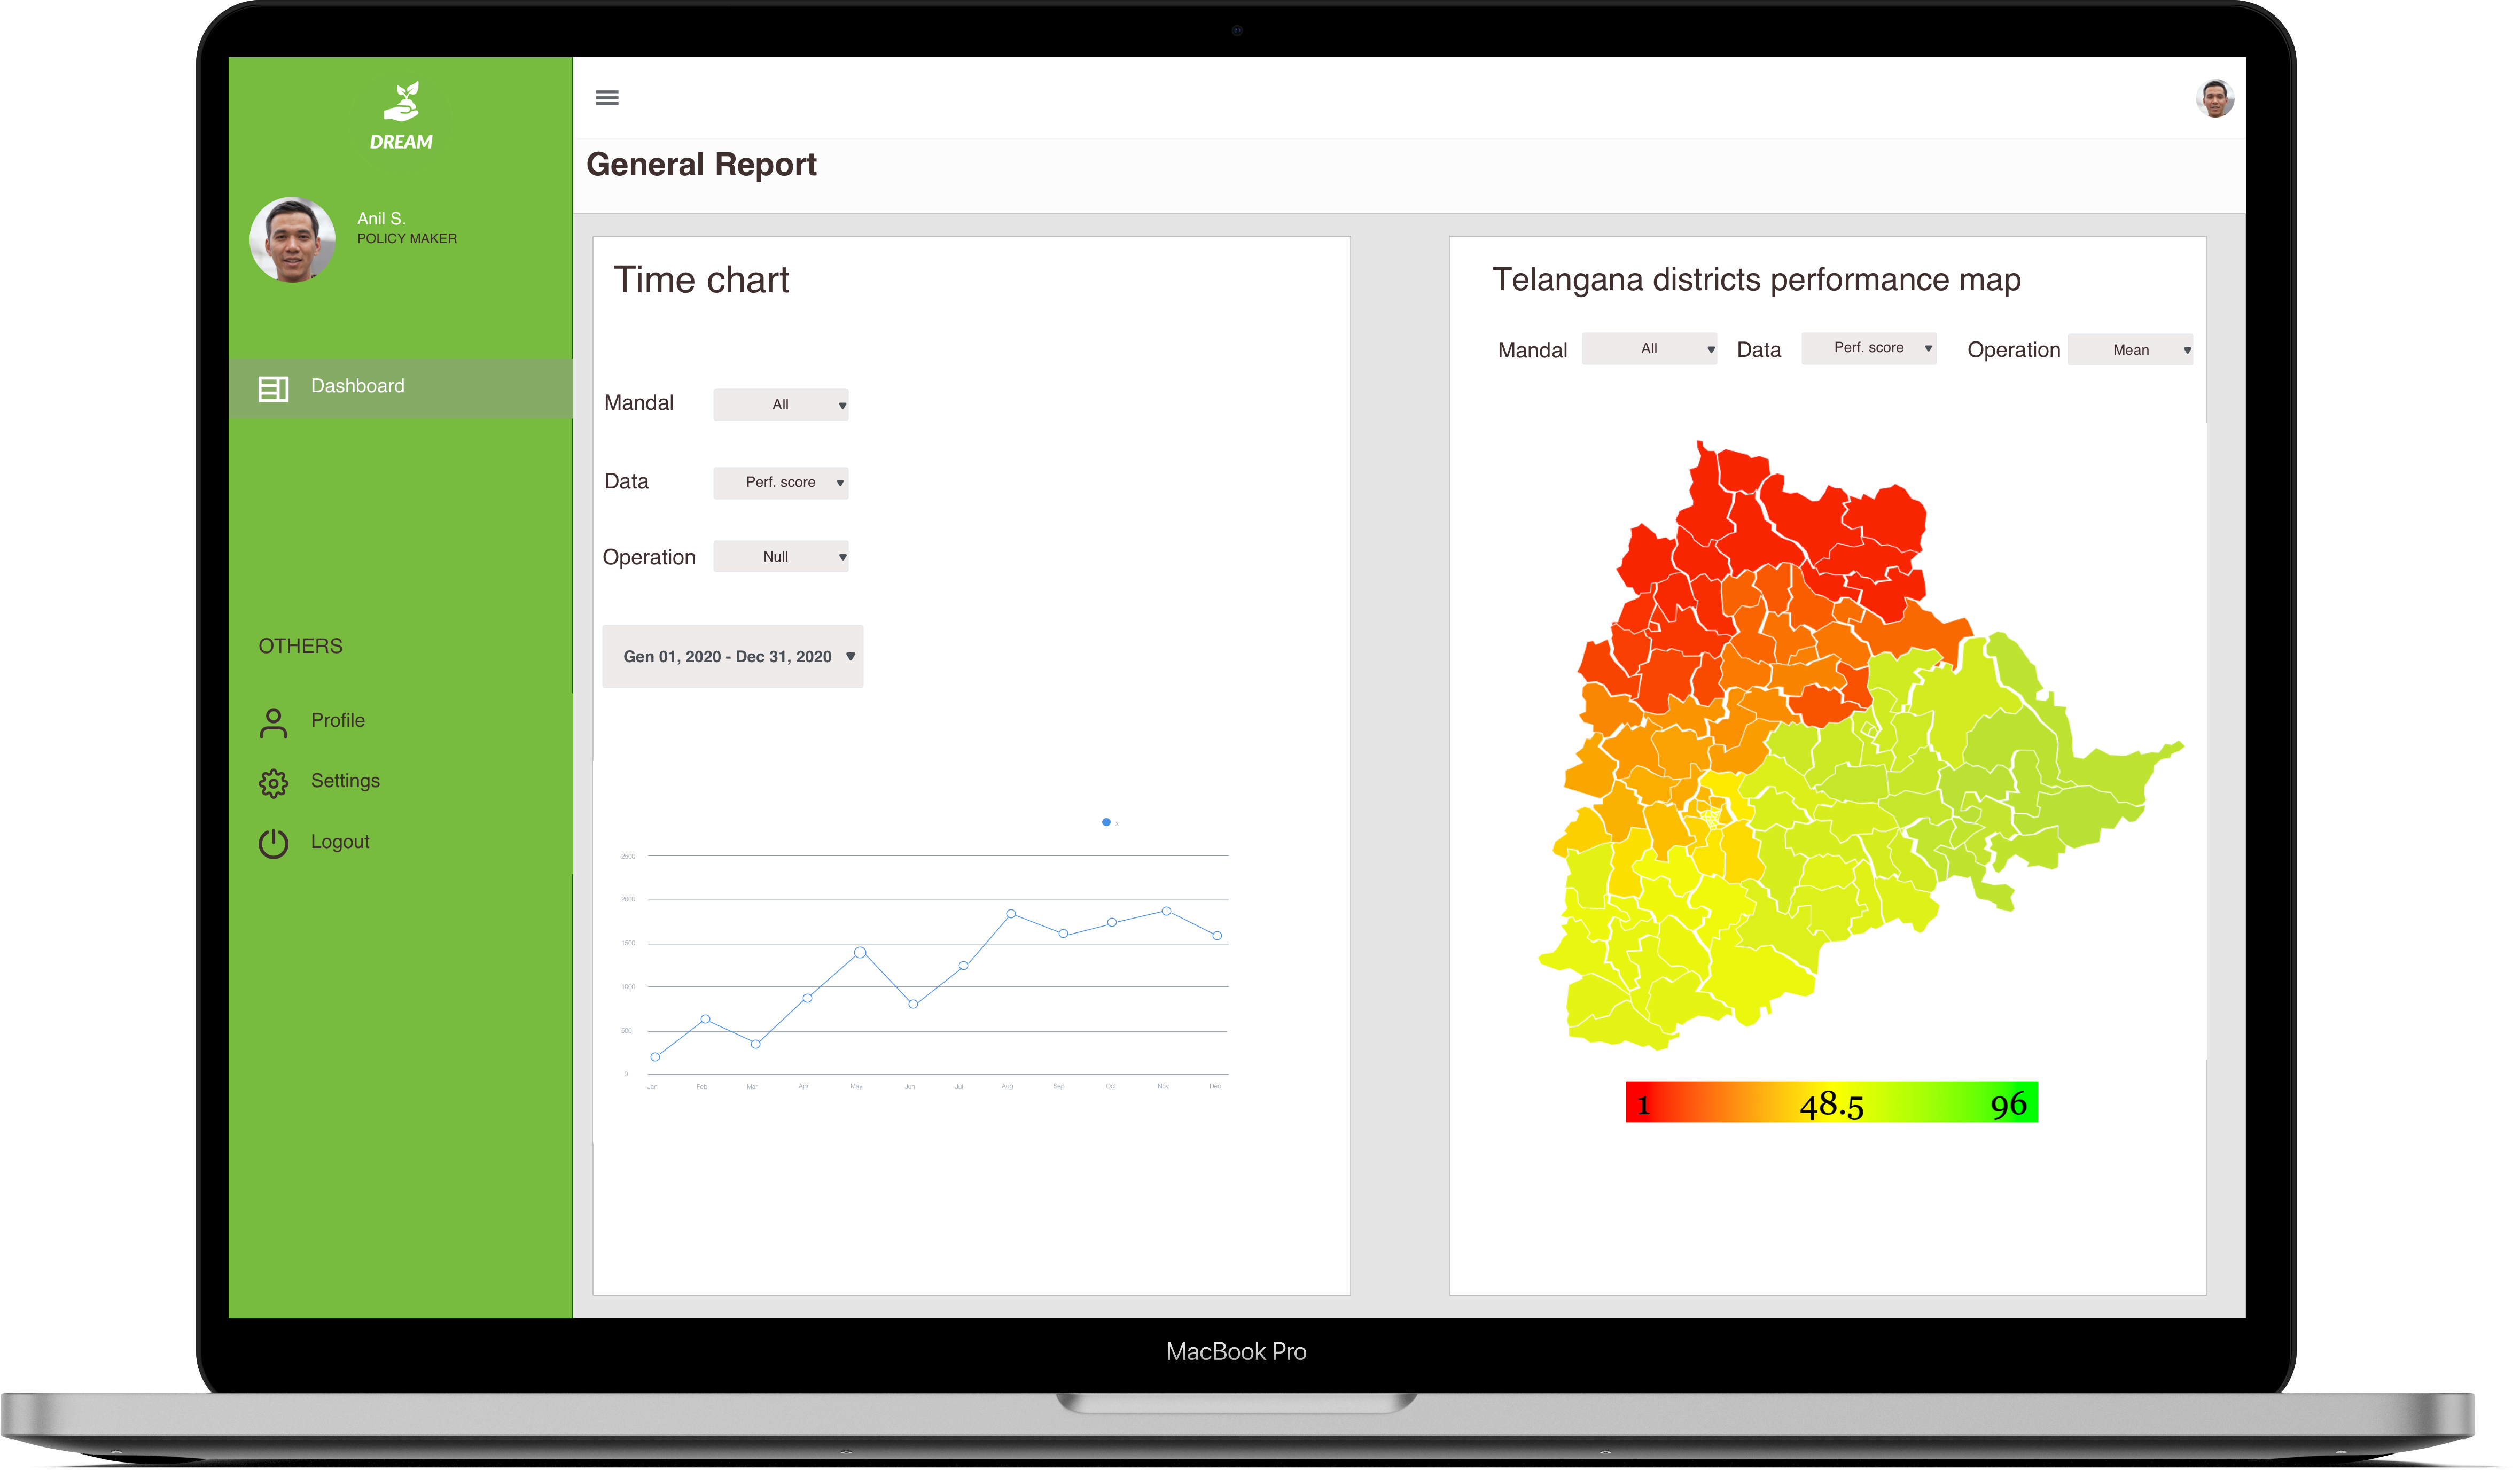
\includegraphics[width=140mm,scale=0.9]{./Images//Mocks/WebApp/PolicyMaker.png}
  \caption{PolicyMaker Homepage}
\end{figure}

\begin{itemize}
    \item \textbf{PolicyMaker Homepage}\\ 
    \textcolor{red}{This is PolicyMaker homepage (in Figure 3.3 called "Dashboard") where the he/she con generate a Time chart according to some inputs, and can also visualize Telangana's farmers performance map.}
\end{itemize}


\begin{figure}[H]
  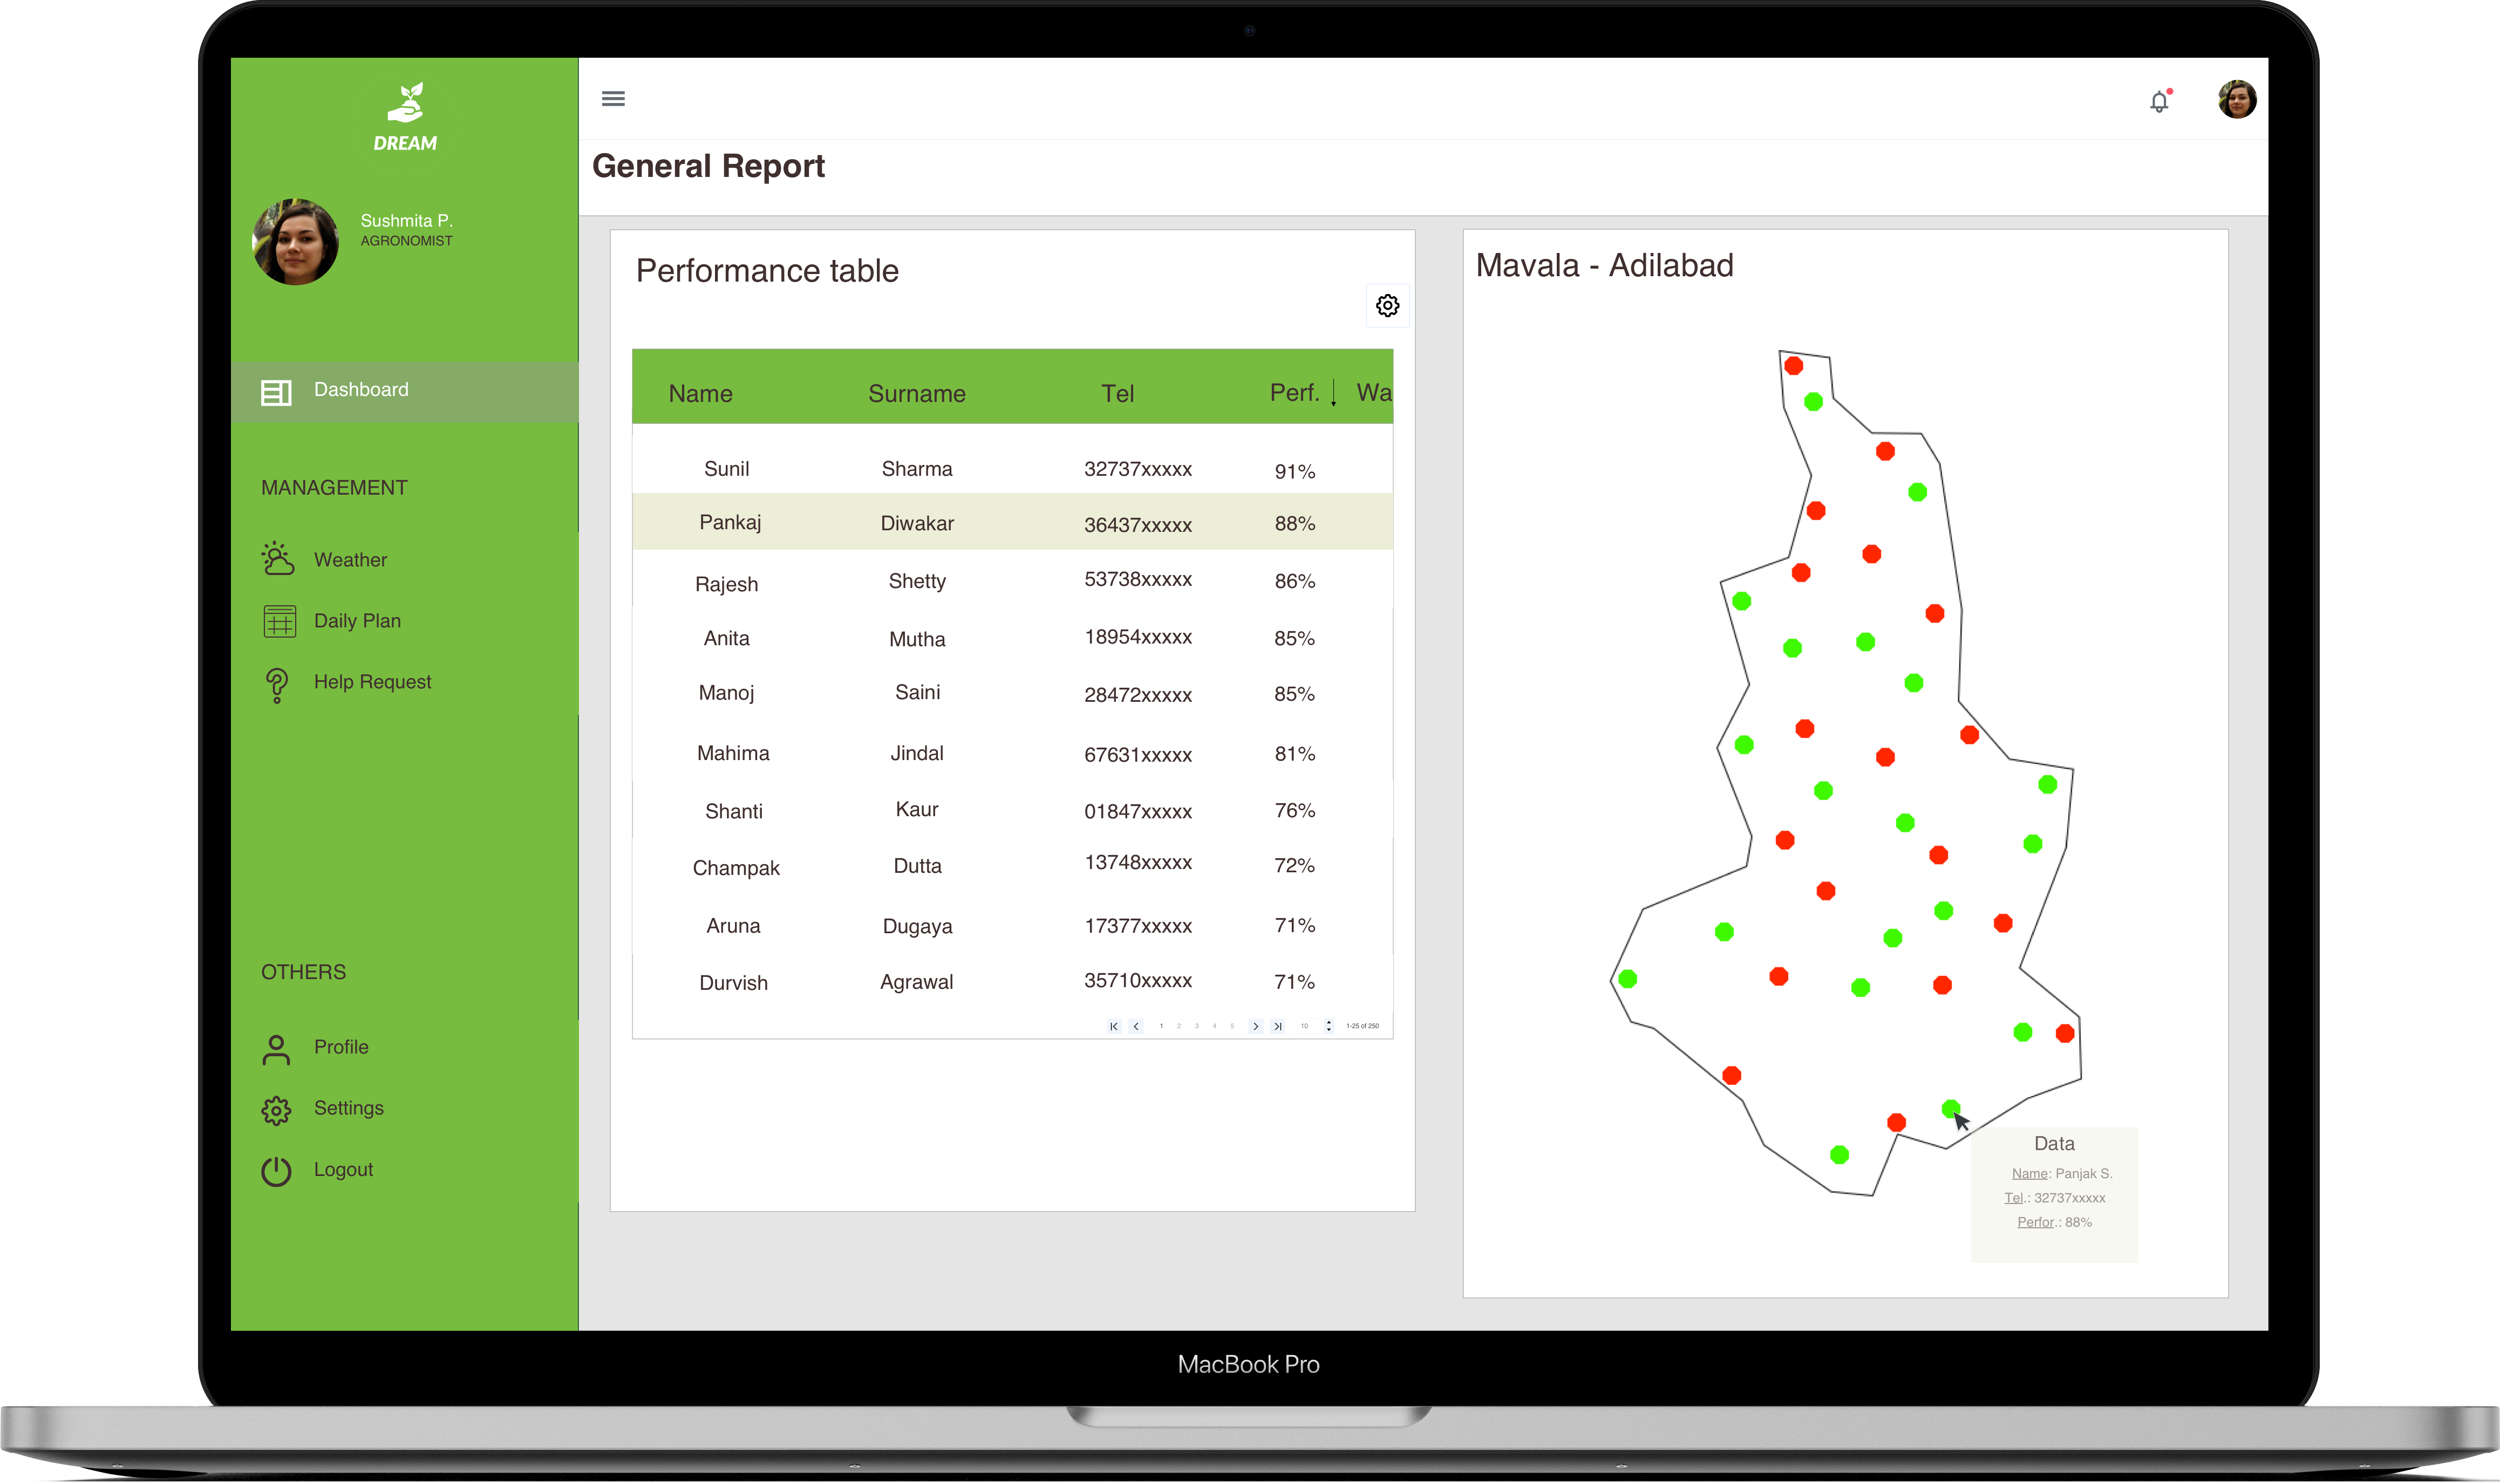
\includegraphics[width=140mm,scale=0.9]{./Images//Mocks/WebApp/Agronomist_Home.png}
  \caption{Agronomist Homepage}
\end{figure}

\begin{itemize}
    \item \textbf{Agronomist Homepage}\\ 
    \textcolor{red}{This is Agronomist homepage (in Figure 3.4 called "Dashboard") where he/she can view his/her mandal's farmer performance and the performance table, that resume, in ascending order (by performance), info's about farmers.}
\end{itemize}


\begin{figure}[H]
  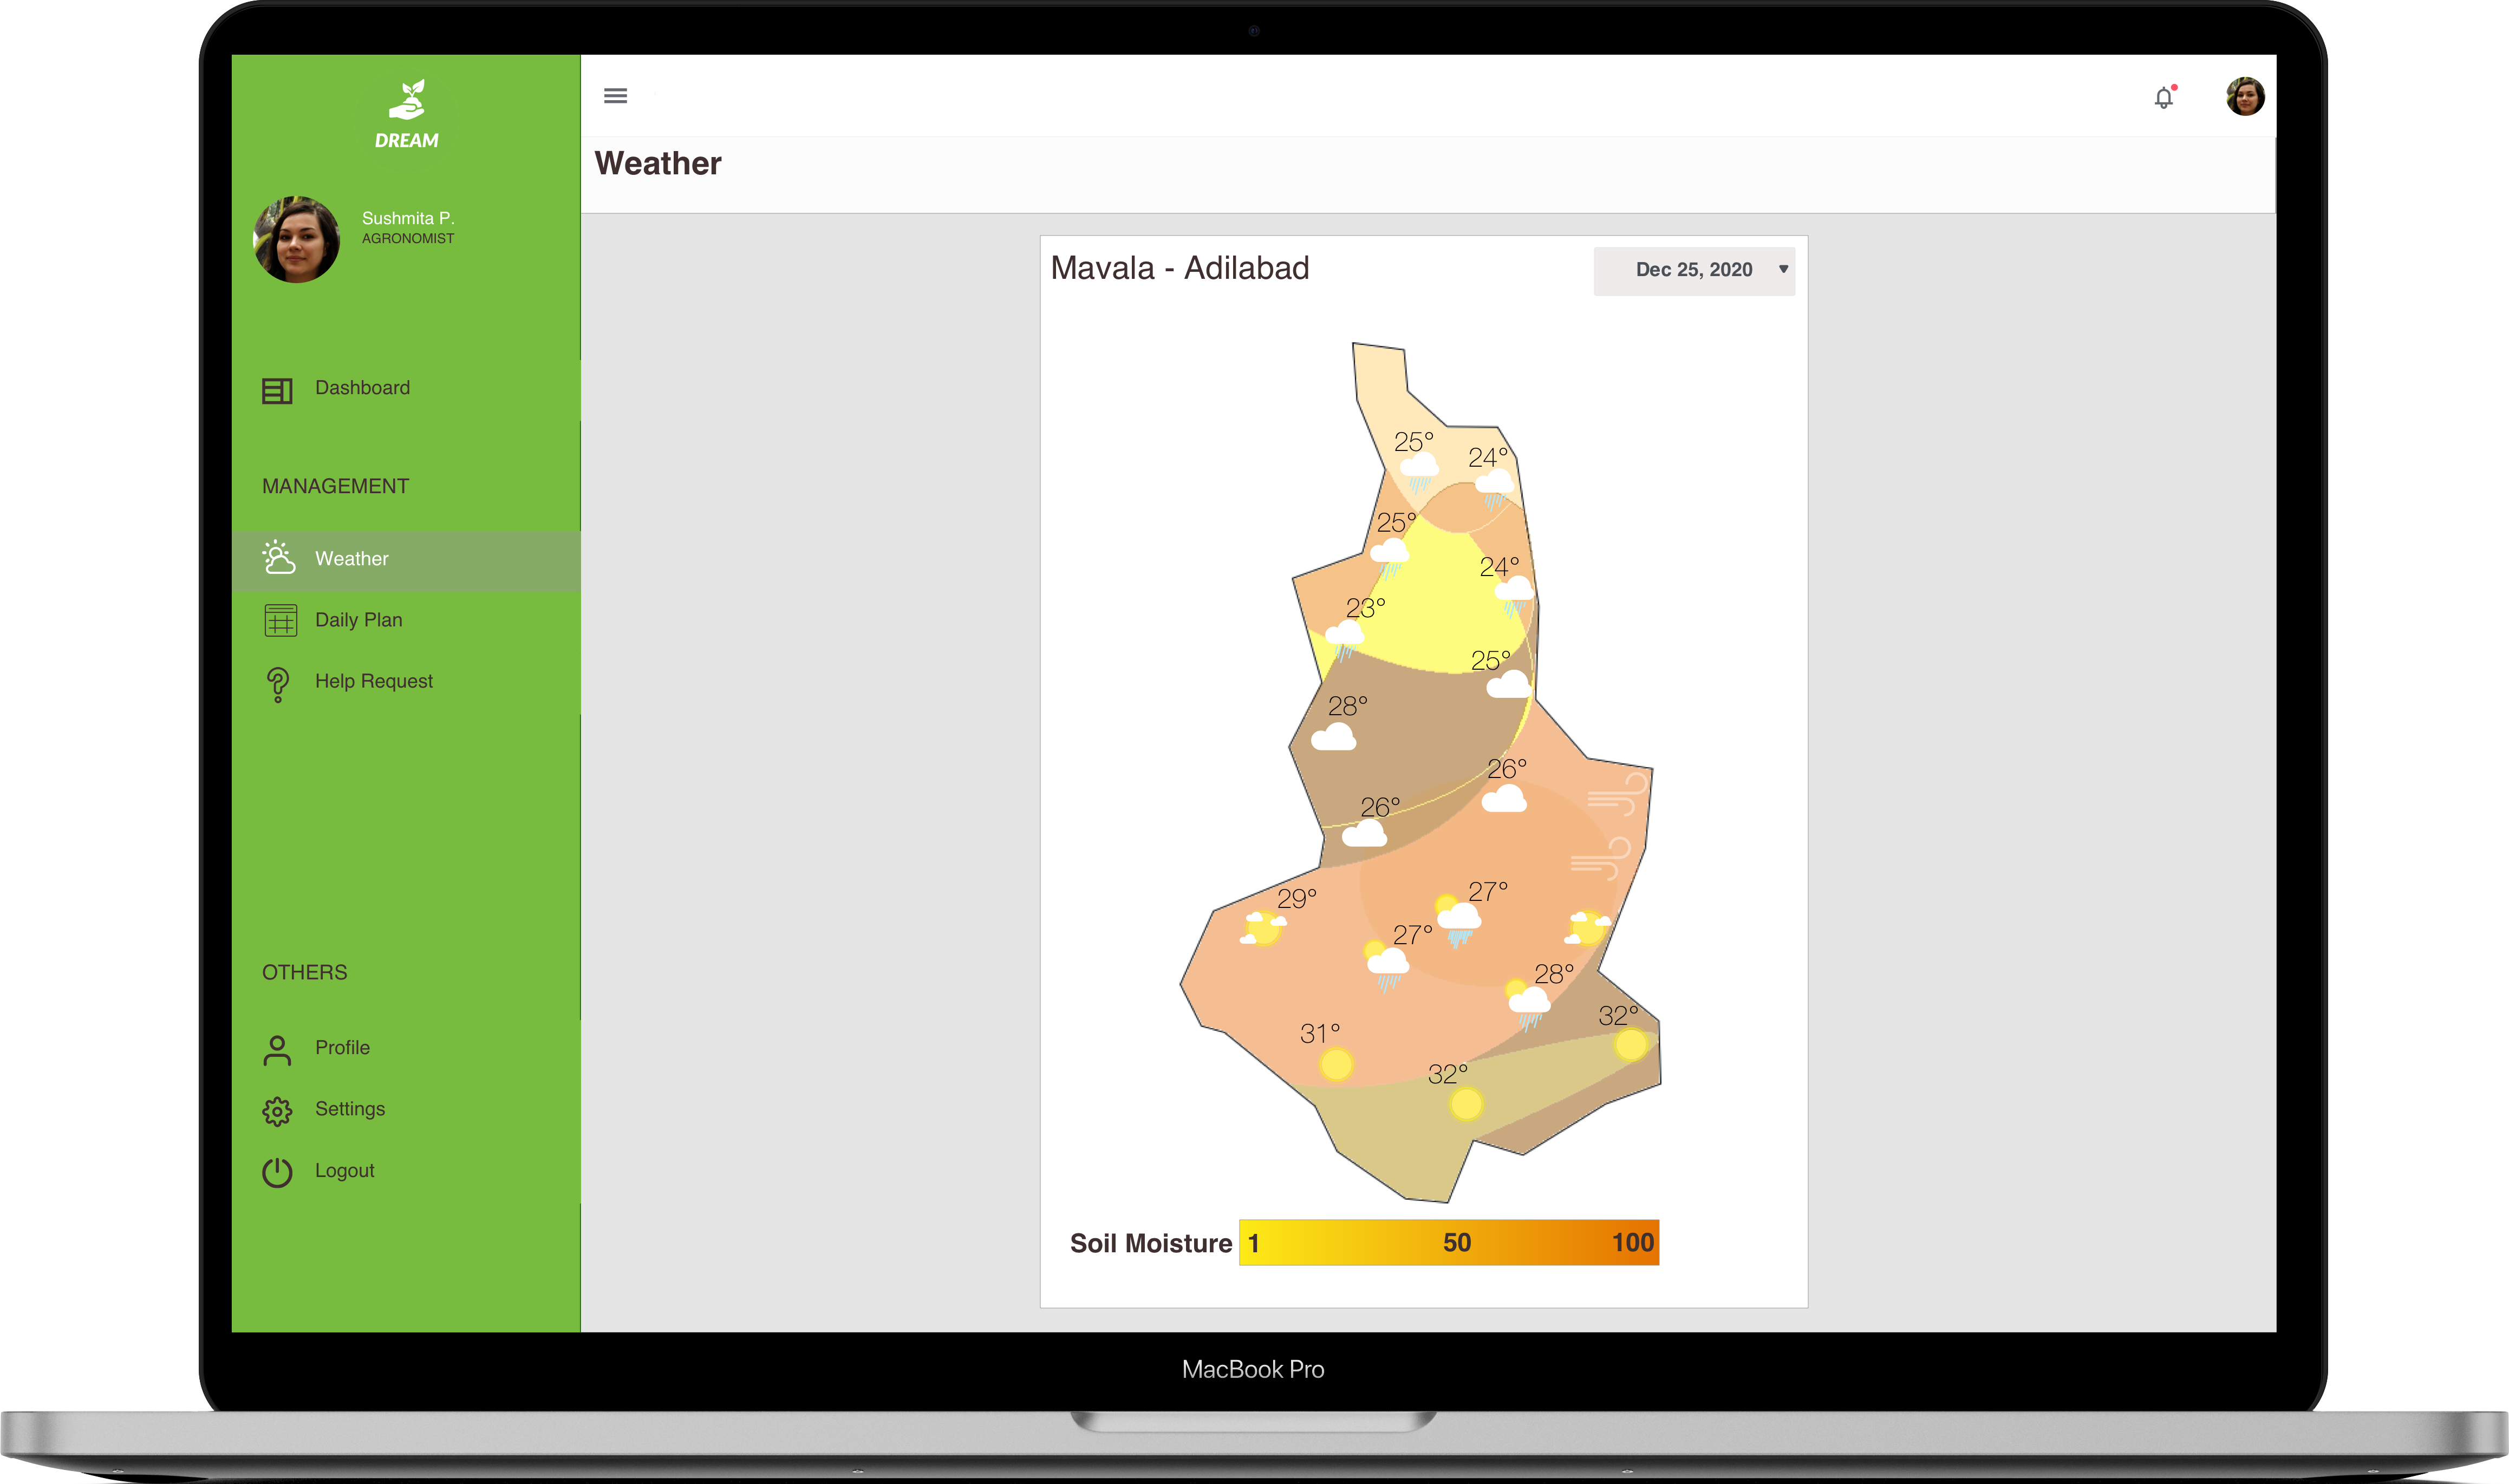
\includegraphics[width=140mm,scale=0.9]{./Images//Mocks/WebApp/Agronomist_Weather.png}
  \caption{Agronomist Weather page}
\end{figure}

\begin{itemize}
    \item \textbf{Agronomist Weather page}\\ 
    \textcolor{red}{This is Agronomist weather page, where he/she can visualize info about weather conditions and soil moisture of his/her mandal}
\end{itemize}


\begin{figure}[H]
  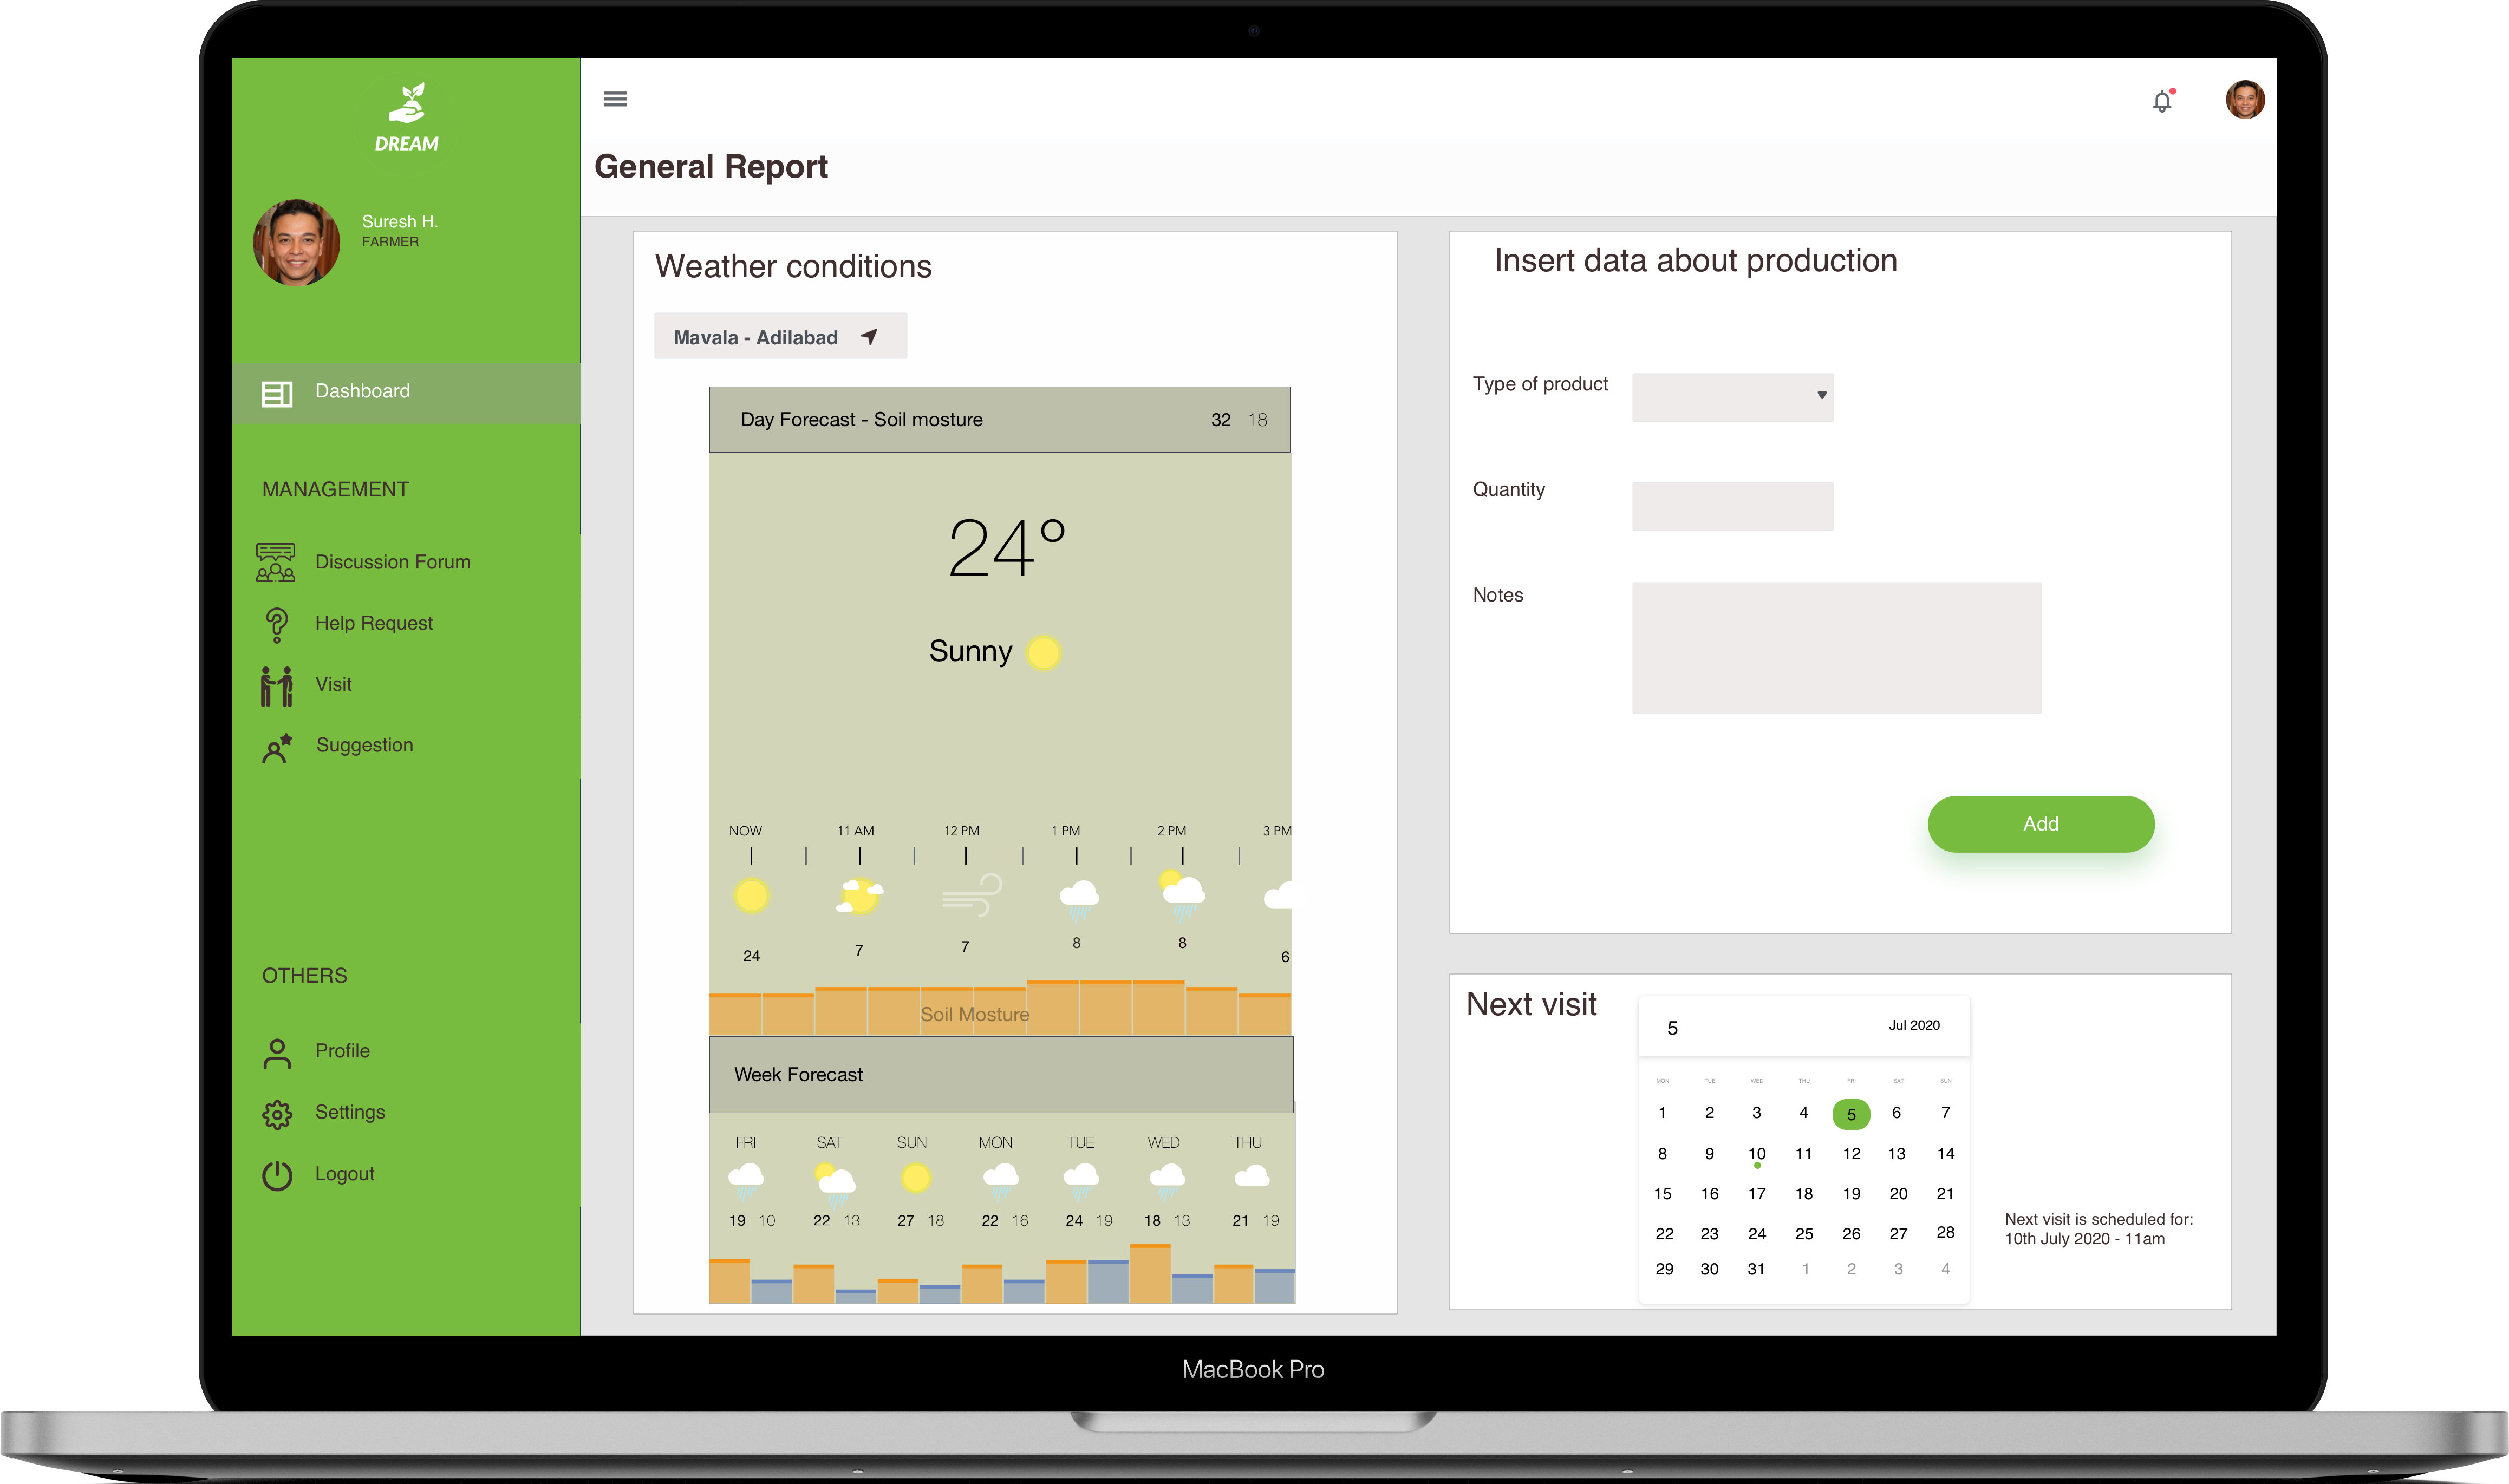
\includegraphics[width=140mm,scale=0.9]{./Images//Mocks/WebApp/Farmer_Home.png}
  \caption{Farmer Home page}
\end{figure}

\begin{itemize}
    \item \textbf{Farmer Home page}\\ 
    \textcolor{red}{This is Farmer homepage (in Figure 3.6 called "Dashboard") where he/she can visualize weather conditions based on her/his location, can insert data about his/her production and can visualize on the calendar the next visit.}
\end{itemize}


\begin{figure}[H]
  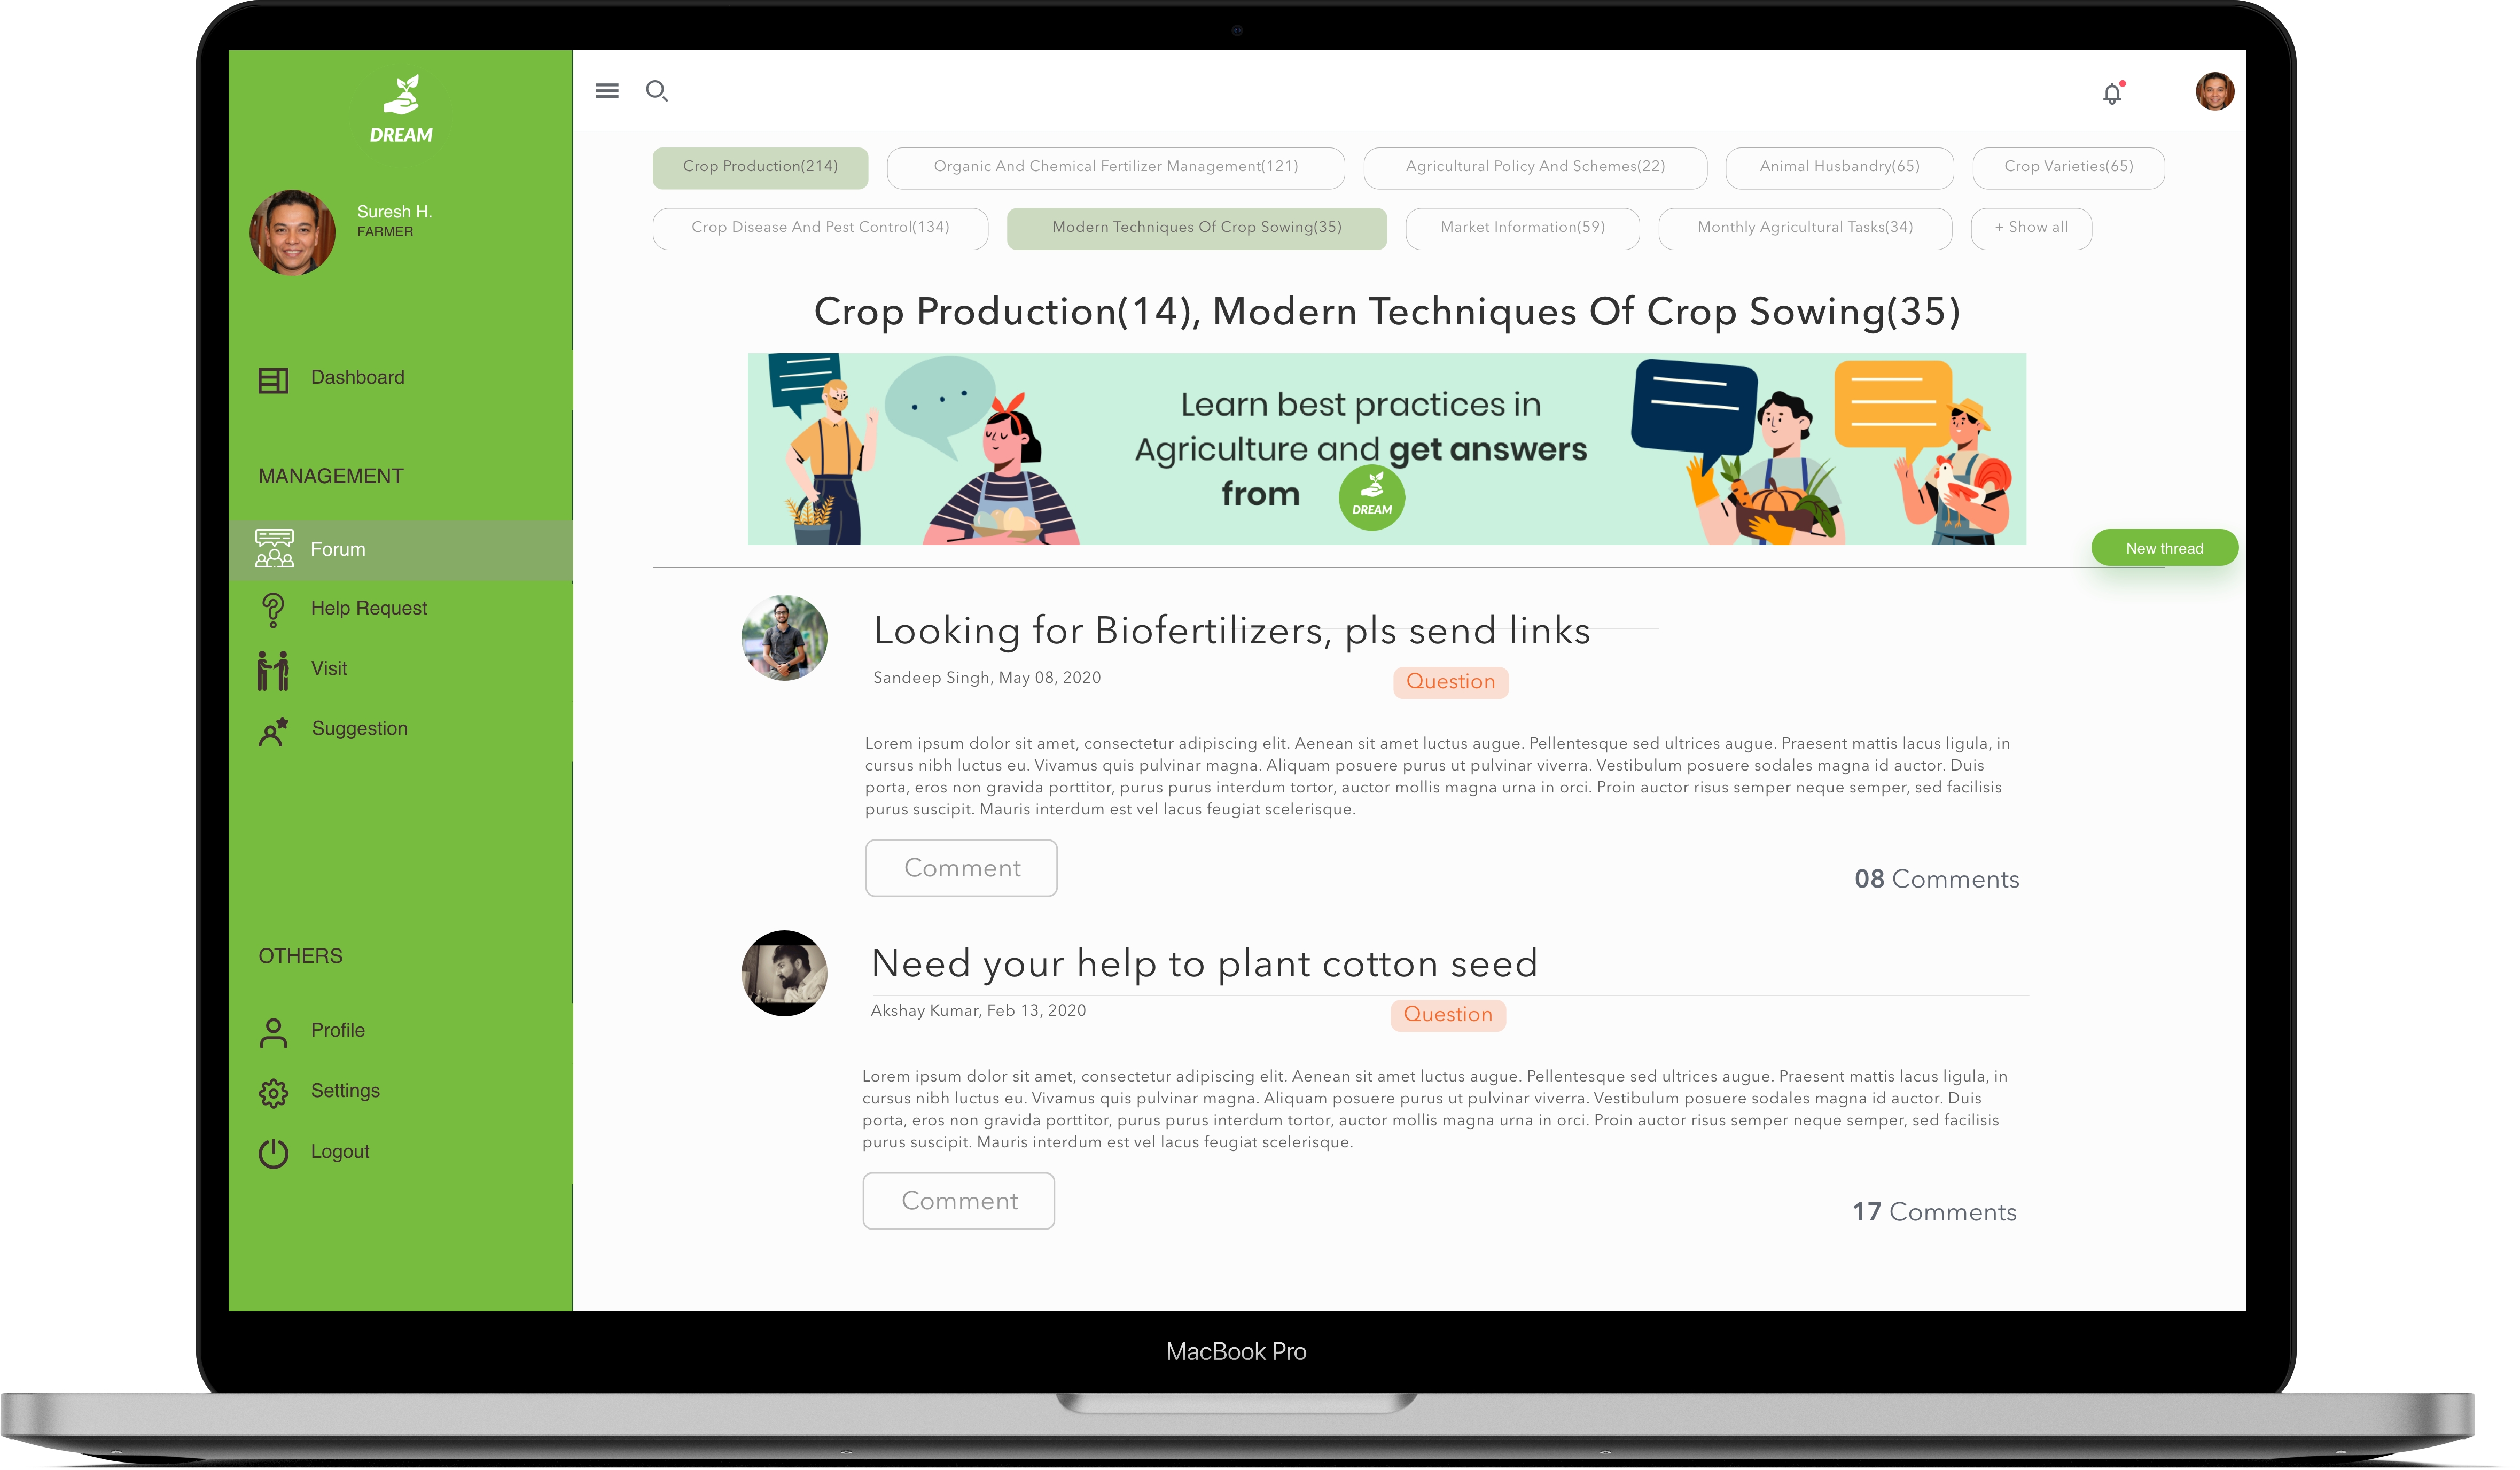
\includegraphics[width=140mm,scale=0.9]{./Images//Mocks/WebApp/Farmer_Forum.png}
  \caption{Farmer Forum page}
\end{figure}

\begin{itemize}
    \item \textbf{Farmer Forum page}\\ 
    \textcolor{red}{This is Farmer forum section, where he can interact with other farmers by opening new threads or replying to existing one.}
\end{itemize}


\begin{figure}[H]
  \centering
  \begin{minipage}{0.4\textwidth}
    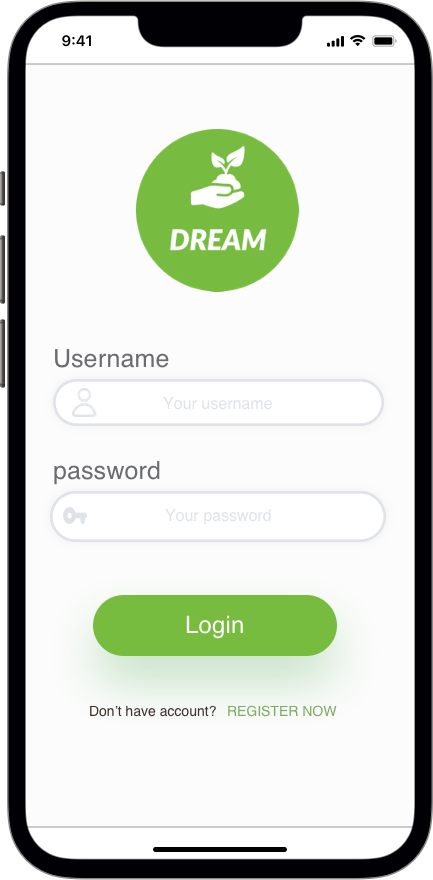
\includegraphics[width=40mm,scale=0.9]{./Images//Mocks/Mobile/Login.png}
    \caption{Mobile Login}
   \end{minipage}
   \hfill
   \begin{minipage}{0.4\textwidth}
     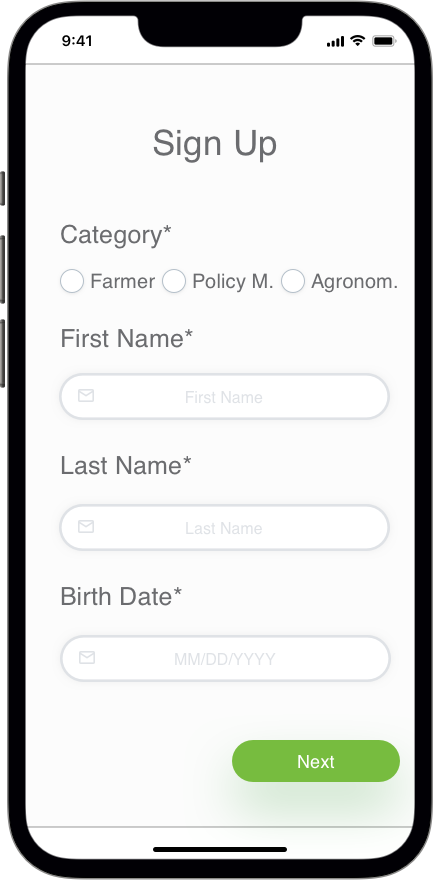
\includegraphics[width=40mm,scale=0.9]{./Images//Mocks/Mobile/Registration.png}
     \caption{Mobile Registration}
   \end{minipage}
\end{figure}


\begin{figure}[H]
  \centering
   \begin{minipage}{0.4\textwidth}
     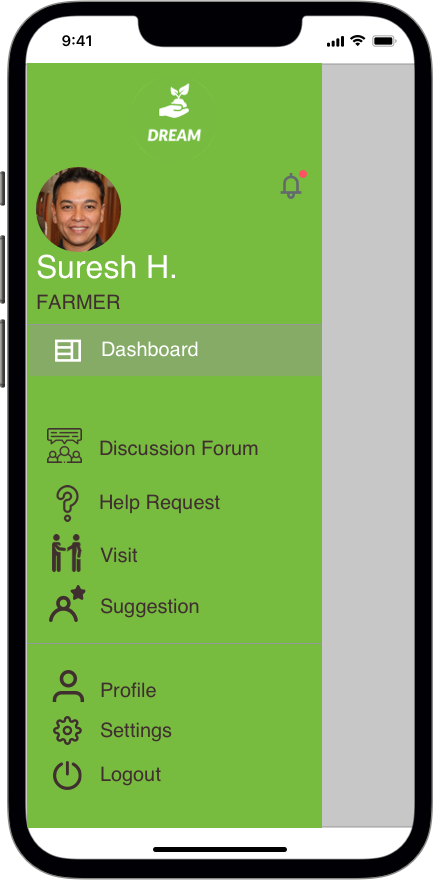
\includegraphics[width=40mm,scale=0.9]{./Images//Mocks/Mobile/Farmer_menu.png}
     \caption{Mobile Farmer menu}
   \end{minipage}
    \hfill
   \begin{minipage}{0.4\textwidth}
     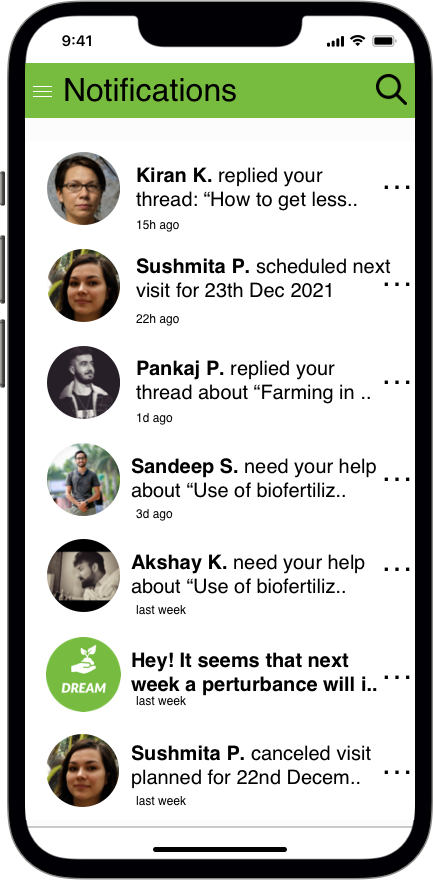
\includegraphics[width=40mm,scale=0.9]{./Images//Mocks/Mobile/Farmer_notif.png}
     \caption{Mobile Farmer notifications}
   \end{minipage}
\end{figure}
\newpage
\begin{itemize}
    \item \textbf{Figure 3.8: Mobile Login}\\ 
    \textcolor{red}{Initial interface, it allows to one of the 3 actors of DREAM to log in by entering their credentials (Username and password)}
\end{itemize}
\begin{itemize}
    \item \textbf{Figure 3.9: Mobile Registration}\\ 
    \textcolor{red}{Through the registration interface, it is possible to create an account by  one of the 3 actors of DREAM.}
\end{itemize}
\begin{itemize}
    \item \textbf{Figure 3.10: Mobile Farmer menu}\\ 
    \textcolor{red}{Interface that shows actions that a farmer can perform in the application}
\end{itemize}
\begin{itemize}
    \item \textbf{Figure 3.11: Mobile Farmer notifications}\\ 
    \textcolor{red}{Interface that shows various kind of notifications received by a Farmer.}
\end{itemize}
\newpage

\begin{figure}[H]
  \centering
   \begin{minipage}{0.4\textwidth}
     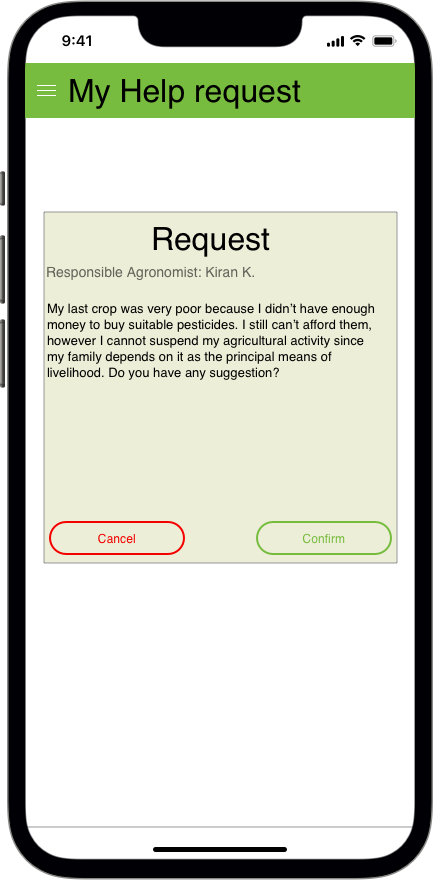
\includegraphics[width=40mm,scale=0.9]{./Images//Mocks/Mobile/Farmer_help_req.png}
     \caption{Mobile Farmer help request}
   \end{minipage}
    \hfill
   \begin{minipage}{0.4\textwidth}
     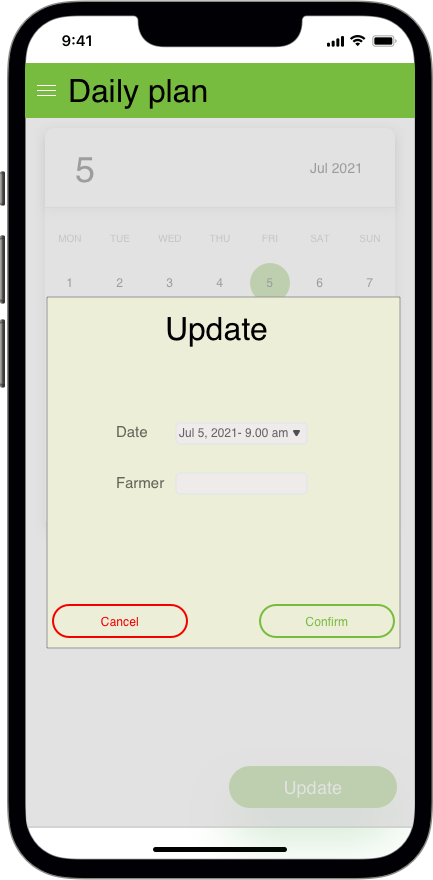
\includegraphics[width=40mm,scale=0.9]{./Images//Mocks/Mobile/Agronomist_daily_plan.png}
     \caption{Mobile Agronomist daily plan}
   \end{minipage}
\end{figure}

\begin{itemize}
    \item \textbf{Figure 3.12: Mobile Farmer help request}\\ 
    \textcolor{red}{Interface that shows an example of help request made by a Farmer to only an Agronomist.}
\end{itemize}
\begin{itemize}
    \item \textbf{Figure 3.13: Mobile Agronomist daily plan}\\ 
    \textcolor{red}{Interface that shows an example of update of the daily plane made by an Agronomist.}
\end{itemize}
\newpage